\pdfoutput=1

In this supplemental material, we include a detailed review of experiment configurations of related work with policy gradient methods in continuous control MuJoCo~\cite{MuJoCo} environment tasks from OpenAI Gym~\cite{gym}. We include a detailed list of the hyperparameters and reported metrics typically used in policy gradient literature in deep RL. We also include all our experimental results, with baseline algorithms DDPG \cite{DDPG}, TRPO \cite{TRPO}, PPO \cite{PPO} and ACKTR \cite{ACKTR}) as discussed in the paper. Our experimental results include figures with different hyperparameters (network architectures, activation functions) to highlight the differences this can have across algorithms and environments.  Finally, as discussed in the paper, we include discussion of significance metrics and show how these metrics can be useful for evaluating deep RL algorithms.


\section{Literature Reviews}

\subsection{Hyperparameters}

In this section, we include a list of hyperparameters that are reported in related literature, as shown in figure \ref{related_work_hyperparams}.  Our analysis shows that often there is no consistency in the type of network architectures and activation functions that are used in related literature. As shown in the paper and from our experimental results in later sections, we find, however, that these hyperparameters can have a significant effect in the performance of algorithms across benchmark environments typically used.

\begin{table}[H]
\centering
\caption{Evaluation Hyperparameters of baseline algorithms reported in related literature}
\label{related_work_hyperparams}
\begin{tabular}{|l|l|l|l|l|l|l|}
\hline
\textbf{\begin{tabular}[c]{@{}l@{}}Related Work\\ (Algorithm)\end{tabular}} & \textbf{\begin{tabular}[c]{@{}l@{}}Policy \\ Network\end{tabular}} & \textbf{\begin{tabular}[c]{@{}l@{}}Policy \\ Network \\ Activation\end{tabular}} & \textbf{\begin{tabular}[c]{@{}l@{}}Value \\ Network\end{tabular}} & \textbf{\begin{tabular}[c]{@{}l@{}}Value\\ Network\\ Activation\end{tabular}} & \textbf{\begin{tabular}[c]{@{}l@{}}Reward\\ Scaling\end{tabular}} & \textbf{\begin{tabular}[c]{@{}l@{}}Batch \\ Size\end{tabular}} \\ \hline
DDPG & 64x64 & ReLU & 64x64 & ReLU & 1.0 & 128 \\ \hline
TRPO & 64x64 & TanH & 64x64 & TanH & - & 5k \\ \hline
PPO & 64x64 & TanH & 64x64 & TanH & - & 2048 \\ \hline
ACKTR & 64x64 & TanH & 64x64 & ELU & - & 2500 \\ \hline
\begin{tabular}[c]{@{}l@{}}Q-Prop\\ (DDPG)\end{tabular} & 100x50x25 & TanH & 100x100 & ReLU & 0.1 & 64 \\ \hline
\begin{tabular}[c]{@{}l@{}}Q-Prop\\ (TRPO)\end{tabular} & 100x50x25 & TanH & 100x100 & ReLU & - & 5k \\ \hline
\begin{tabular}[c]{@{}l@{}}IPG\\ (TRPO)\end{tabular} & 100x50x25 & TanH & 100x100 & ReLU & - & 10k \\ \hline
\begin{tabular}[c]{@{}l@{}}Param Noise\\ (DDPG)\end{tabular} & 64x64 & ReLU & 64x64 & ReLU & - & 128 \\ \hline
\begin{tabular}[c]{@{}l@{}}Param Noise\\ (TRPO)\end{tabular} & 64x64 & TanH & 64x64 & TanH & - & 5k \\ \hline
\begin{tabular}[c]{@{}l@{}}Benchmarking\\ (DDPG)\end{tabular} & 400x300 & ReLU & 400x300 & ReLU & 0.1 & 64 \\ \hline
\begin{tabular}[c]{@{}l@{}}Benchmarking\\ (TRPO)\end{tabular} & 100x50x25 & TanH & 100x50x25 & TanH & - & 25k \\ \hline
\end{tabular}
\end{table}


\subsection{Reported Results on Benchmarked Environments}

We then demonstrate how experimental reported results, on two different environments (HalfCheetah-v1 and Hopper-v1) can vary across different related work that uses these algorithms for baseline comparison. We further show the results we get, using the same hyperparameter configuration, but using two different codebase implementations (note that these implementations are often used as baseline codebase to develop algorithms). We highlight that, depending on the codebase used, experimental results can vary significantly.


\begin{table}[H]
\centering
\caption{Comparison with Related Reported Results with Hopper Environment}
\label{tab:comparison_baseline_results2}
\small{\begin{tabular}{llllllll}
Environment & Metric & rllab  & QProp & IPG  & TRPO & \begin{tabular}[c]{@{}l@{}}Our Results\\ (rllab)\end{tabular} & \begin{tabular}[c]{@{}l@{}}Our Results \\ (Baselines)\end{tabular}\\
\multirow{3}{*}{\begin{tabular}[c]{@{}l@{}}TRPO on\\ Hopper\\ Environment\end{tabular}}
& Number of Iterations & 500    & 500   & 500  & 500  & 500 & 500 \\
& Average Return & 1183.3  &  -  &  -   &   -  & 2021.34  &  2965.3\\
& Max Average Return & - & 2486   &  & 3668.8  &  3229.1  &  3034.4\\
\end{tabular}}
\end{table}


\begin{table}[H]
\centering
\caption{Comparison with Related Reported Results with HalfCheetah Environment}
\label{tab:comparison_baseline_results}
\small{\begin{tabular}{llllllll}
Environment & Metric & rllab  & QProp & IPG  & TRPO & \begin{tabular}[c]{@{}l@{}}Our Results\\ (rllab)\end{tabular} & \begin{tabular}[c]{@{}l@{}}Our Results \\ (Baselines)\end{tabular}\\
\multirow{3}{*}{\begin{tabular}[c]{@{}l@{}}TRPO on\\ HalfCheetah\\ Environment\end{tabular}}
& Number of Iterations & 500    & 500   & 500  & 500  & 500 & 500 \\
& Average Return & 1914.0 &    & -    & -    & 3576.08 & 1045.6 \\
& Max Average Return   & -      & 4734  & 2889 & 4855 & 5197 & 1045.6\\
\end{tabular}}
\end{table}

\begin{table}[H]
    \centering
    \begin{tabular}{c|c}
         \hline
         Work & Number of Trials \\
         \hline
         \cite{mnih2016asynchronous}& top-5\\
         \cite{PPO} & 3-9 \\
         \cite{rllab} & 5 (5)\\
         \cite{IPG} & 3\\
         \cite{DDPG} & 5\\
         \cite{TRPO} & 5\\
         \cite{ACKTR} & top-2, top-3\\
         \hline
    \end{tabular}
    \caption{Number of trials reported during evaluation in various works.}
    \label{tab:trials}
\end{table}

\subsection{Reported Evaluation Metrics in Related Work}

In table \ref{reported_eval_metric} we show the evaluation metrics, and reported results in further details across related work.


\begin{table}[H]
\centering
\caption{Reported Evaluation Metrics of baseline algorithms in related literature}
\label{reported_eval_metric}
\begin{tabular}{|c|c|c|c|c|c|}
\hline
\textbf{\begin{tabular}[c]{@{}c@{}}Related Work\\ (Algorithm)\end{tabular}} & \textbf{Environments} & \textbf{\begin{tabular}[c]{@{}c@{}}Timesteps\\ or Episodes\\ or Iterations\end{tabular}} & \multicolumn{3}{c|}{\textbf{Evaluation Metrics}} \\ \hline
 &  &  & \textbf{\begin{tabular}[c]{@{}c@{}}Average \\ Return\end{tabular}} & \textbf{\begin{tabular}[c]{@{}c@{}}Max \\ Return\end{tabular}} & \textbf{\begin{tabular}[c]{@{}c@{}}Std \\ Error\end{tabular}} \\ \hline
PPO & \begin{tabular}[c]{@{}c@{}}HalfCheetah\\ Hopper\end{tabular} & 1M & \begin{tabular}[c]{@{}c@{}}$\sim$1800\\ $\sim$2200\end{tabular} & - & - \\ \hline
ACKTR & \begin{tabular}[c]{@{}c@{}}HalfCheetah\\ Hopper\end{tabular} & 1M & \begin{tabular}[c]{@{}c@{}}$\sim$2400\\ $\sim$3500\end{tabular} & - & - \\ \hline
\begin{tabular}[c]{@{}c@{}}Q-Prop\\ (DDPG)\end{tabular} & \begin{tabular}[c]{@{}c@{}}HalfCheetah\\ Hopper\end{tabular} & 6k (eps) & \begin{tabular}[c]{@{}c@{}}$\sim$6000\\ -\end{tabular} & \begin{tabular}[c]{@{}c@{}}7490\\ 2604\end{tabular} & \begin{tabular}[c]{@{}c@{}}-\\ -\end{tabular} \\ \hline
\begin{tabular}[c]{@{}c@{}}Q-Prop\\ (TRPO)\end{tabular} & \begin{tabular}[c]{@{}c@{}}HalfCheetah\\ Hopper\end{tabular} & 5k (timesteps) & \begin{tabular}[c]{@{}c@{}}$\sim$4000\\ -\end{tabular} & \begin{tabular}[c]{@{}c@{}}4734\\ 2486\end{tabular} & \begin{tabular}[c]{@{}c@{}}-\\ -\end{tabular} \\ \hline
\begin{tabular}[c]{@{}c@{}}IPG\\ (TRPO)\end{tabular} & \begin{tabular}[c]{@{}c@{}}HalfCheetah\\ Hopper\end{tabular} & 10k (eps) & \begin{tabular}[c]{@{}c@{}}$\sim$3000\\ -\end{tabular} & 2889 & \begin{tabular}[c]{@{}c@{}}-\\ -\end{tabular} \\ \hline
\begin{tabular}[c]{@{}c@{}}Param Noise\\ (DDPG)\end{tabular} & \begin{tabular}[c]{@{}c@{}}HalfCheetah\\ Hopper\end{tabular} & 1M & \begin{tabular}[c]{@{}c@{}}$\sim$1800\\ $\sim$500\end{tabular} & \begin{tabular}[c]{@{}c@{}}-\\ -\end{tabular} & \begin{tabular}[c]{@{}c@{}}-\\ -\end{tabular} \\ \hline
\begin{tabular}[c]{@{}c@{}}Param Noise\\ (TRPO)\end{tabular} & \begin{tabular}[c]{@{}c@{}}HalfCheetah\\ Hopper\end{tabular} & 1M & \begin{tabular}[c]{@{}c@{}}$\sim$3900\\ $\sim$2400\end{tabular} & \begin{tabular}[c]{@{}c@{}}-\\ -\end{tabular} & \begin{tabular}[c]{@{}c@{}}-\\ -\end{tabular} \\ \hline
\begin{tabular}[c]{@{}c@{}}Benchmarking\\ (DDPG)\end{tabular} & \begin{tabular}[c]{@{}c@{}}HalfCheetah\\ Hopper\end{tabular} & \begin{tabular}[c]{@{}c@{}}500 iters\\ (25k eps)\end{tabular} & \begin{tabular}[c]{@{}c@{}}$\sim$2148\\ $\sim$267\end{tabular} & \begin{tabular}[c]{@{}c@{}}-\\ -\end{tabular} & \begin{tabular}[c]{@{}c@{}}702\\ 43\end{tabular} \\ \hline
\begin{tabular}[c]{@{}c@{}}Benchmarking\\ (TRPO)\end{tabular} & \begin{tabular}[c]{@{}c@{}}HalfCheetah\\ Hopper\end{tabular} & \begin{tabular}[c]{@{}c@{}}500 iters\\ (925k eps)\end{tabular} & \begin{tabular}[c]{@{}c@{}}$\sim$1914\\ $\sim$1183\end{tabular} & \begin{tabular}[c]{@{}c@{}}-\\ -\end{tabular} & \begin{tabular}[c]{@{}c@{}}150\\ 120\end{tabular} \\ \hline
\end{tabular}
\end{table}





\section{Experimental Setup}

In this section, we show detailed analysis of our experimental results, using same hyperparameter configurations used in related work.  Experimental results are included for the OpenAI Gym~\cite{gym} Hopper-v1 and HalfCheetah-v1 environments, using the  policy gradient algorithms including DDPG, TRPO, PPO and ACKTR. Our experiments are done using the available codebase from OpenAI rllab \cite{rllab} and OpenAI Baselines. Each of our experiments are performed over 5 experimental trials with different random seeds, and results averaged over all trials. Unless explicitly specified as otherwise (such as in hyperparameter modifications where we alter a hyperparameter under investigation), hyperparameters were as follows. All results (including graphs) show mean and standard error across random seeds.

\begin{itemize}
    \item DDPG
    \begin{itemize}
        \item Policy Network: (64, relu, 64, relu, tanh); Q Network (64, relu, 64, relu, linear)
        \item Normalized observations with running mean filter
        \item Actor LR: $1e-4$; Critic LR: $1e-3$
        \item Reward Scale: 1.0
        \item Noise type: O-U 0.2
        \item Soft target update $\tau=.01$
        \item $\gamma=0.995$
        \item batch size = 128
        \item Critic L2 reg $1e-2$
    \end{itemize}
    \item PPO
    \begin{itemize}
        \item Policy Network: (64, tanh, 64, tanh, Linear) + Standard Deviation variable; Value Network (64, tanh, 64, tanh, linear)
        \item Normalized observations with running mean filter
        \item Timesteps per batch 2048
        \item clip param = 0.2
        \item entropy coeff = 0.0
        \item Optimizer epochs per iteration = 10
        \item Optimizer step size $3e-4$
        \item Optimizer batch size 64
        \item Discount $\gamma=0.995$, GAE $\lambda=0.97$
        \item learning rate schedule is constant
    \end{itemize}
    \item TRPO
    \begin{itemize}
        \item Policy Network: (64, tanh, 64, tanh, Linear) + Standard Deviation variable; Value Network (64, tanh, 64, tanh, linear)
        \item Normalized observations with running mean filter
        \item Timesteps per batch 5000
        \item max KL=0.01
        \item Conjugate gradient iterations = 20
        \item CG damping = 0.1
        \item VF Iterations = 5
        \item VF Batch Size = 64
        \item VF Step Size = $1e-3$
        \item entropy coeff = 0.0
        \item Discount $\gamma=0.995$, GAE $\lambda=0.97$
    \end{itemize}
    \item ACKTR
    \begin{itemize}
        \item Policy Network: (64, tanh, 64, tanh, Linear) + Standard Deviation variable; Value Network (64, elu, 64, elu, linear)
        \item Normalized observations with running mean filter
        \item Timesteps per batch 2500
        \item desired KL = .002
        \item Discount $\gamma=0.995$, GAE $\lambda=0.97$
    \end{itemize}
\end{itemize}


\subsection{Modifications to Baseline Implementations}
To ensure fairness of comparison, we make several modifications to the existing implementations. First, we change evaluation in DDPG~\cite{plappert2017parameter} such that during evaluation at the end of an epoch, 10 full trajectories are evaluated. In the current implementation, only a partial trajectory is evaluated immediately after training such that a full trajectory will be evaluated across several different policies, this corresponds more closely to the online view of evaluation, while we take a policy optimization view when evaluating algorithms.

\subsection{Hyperparameters : Network Structures and Activation Functions}
\noindent
Below, we examine the significance of the network configurations used for the non-linear function approximators in policy gradient methods. Several related work have used different sets of network configurations (network sizes and activation functions). We use the reported network configurations from other works, and demonstrate the significance of careful fine tuning that is required.  We demonstrate results using the network activation functions, ReLU, TanH and Leaky ReLU, where most papers use ReLU and TanH as activation functions without detailed reporting of the effect of these activation functions. We analyse the signifcance of using different activations in the policy and action value networks. Previously, we included a detailed table showing average reward with standard error obtained for each of the hyperparameter configurations. In the results below, we show detailed results of how each of these policy gradient algorithms are affected by the choice of the network configuration.

\subsection{Proximal Policy Optimization (PPO)}

\begin{figure}[H]
    \centering
    \includegraphics[width=.49\textwidth]{"images/HalfCheetah-v1__PPO,_Policy_Network_Activation_"}
    \includegraphics[width=.49\textwidth]{"images/Hopper-v1__PPO,_Policy_Network_Activation_"}
    \includegraphics[width=.49\textwidth]{"images/HalfCheetah-v1__PPO,_Value_Network_Activation_"}
    \includegraphics[width=.49\textwidth]{"images/Hopper-v1__PPO,_Value_Network_Activation_"}

    \caption{PPO Policy and Value Network activation}
    \label{fig:pponetworkact}
\end{figure}

\noindent
Experiment results in Figure \ref{fig:pponetworkact}, \ref{fig:pponetwork2}, and \ref{fig:pponetwork} in this section show the effect of the policy network structures and activation functions in the Proximal Policy Optimization (PPO) algorithm.

\begin{figure}[H]
    \centering
    \includegraphics[width=.49\textwidth]{"images/HalfCheetah-v1__PPO,_Policy_Network_Structure_"}
    \includegraphics[width=.49\textwidth]{"images/Hopper-v1__PPO,_Policy_Network_Structure_"}
    \caption{PPO Policy Network structure}
    \label{fig:pponetwork2}
\end{figure}

\begin{figure}[H]
    \includegraphics[width=.49\textwidth]{"images/HalfCheetah-v1__PPO,_Value_Network_Structure_"}
    \includegraphics[width=.49\textwidth]{"images/Hopper-v1__PPO,_Value_Network_Structure_"}
    \caption{PPO Value Network structure}
    \label{fig:pponetwork}
\end{figure}





\subsection{Actor Critic using
Kronecker-Factored Trust Region (ACKTR)}

\begin{figure}[H]
    \centering
    \includegraphics[width=.49\textwidth]{"images/HalfCheetah-v1__ACKTR,_Policy_Network_Structure_"}
    \includegraphics[width=.49\textwidth]{"images/Hopper-v1__ACKTR,_Policy_Network_Structure_"}
    \caption{ACKTR Policy Network structure}
    \label{fig:acktrnetwork3}
\end{figure}

\begin{figure}[H]
    \centering
    \includegraphics[width=.49\textwidth]{"images/HalfCheetah-v1__ACKTR,_Value_Network_Structure_"}
    \includegraphics[width=.49\textwidth]{"images/Hopper-v1__ACKTR,_Value_Network_Structure_"}
    \caption{ACKTR Value Network structure}
    \label{fig:acktrnetwork2}
\end{figure}


\begin{figure}[H]
    \centering
    \includegraphics[width=.49\textwidth]{"images/HalfCheetah-v1__ACKTR,_Policy_Network_Activation_"}
    \includegraphics[width=.49\textwidth]{"images/Hopper-v1__ACKTR,_Policy_Network_Activation_"}
    \caption{ACKTR Policy Network Activation}
    \label{fig:acktrnetwork4}
  \end{figure}

\begin{figure}[H]
    \centering
    \includegraphics[width=.49\textwidth]{"images/HalfCheetah-v1__ACKTR,_Value_Network_Activation_"}
    \includegraphics[width=.49\textwidth]{"images/Hopper-v1__ACKTR,_Value_Network_Activation_"}
    \caption{ACKTR Value Network Activation}
    \label{fig:acktrnetworkact}
\end{figure}

We then similarly, show the significance of these hyperparameters in the ACKTR algorithm. Our results show that the value network structure can have a significant effect on the performance of ACKTR algorithm.

\subsection{Trust Region Policy Optimization (TRPO)}
\noindent
\begin{figure}[H]
    \centering
    \includegraphics[width=.49\textwidth]{"images/HalfCheetah-v1__TRPO,_Policy_Network_Structure_"}
    \includegraphics[width=.49\textwidth]{"images/Hopper-v1__TRPO,_Policy_Network_Structure_"}
    \caption{TRPO Policy Network structure}
    \label{fig:trponetwork2}
  \end{figure}

\begin{figure}[H]
    \centering
    \includegraphics[width=.49\textwidth]{"images/HalfCheetah-v1__TRPO,_Value_Network_Structure_"}
    \includegraphics[width=.49\textwidth]{"images/Hopper-v1__TRPO,_Value_Network_Structure_"}
    \caption{TRPO Value Network structure}
    \label{fig:trponetwork}
\end{figure}

\begin{figure}[H]
    \centering
    \includegraphics[width=.49\textwidth]{"images/HalfCheetah-v1__TRPO,_Policy_Network_Activation_"}
    \includegraphics[width=.49\textwidth]{"images/Hopper-v1__TRPO,_Policy_Network_Activation_"}
    \caption{TRPO Policy and Value Network activation}
    \label{fig:trponetwork3}
  \end{figure}

\begin{figure}[H]
  \centering
    \includegraphics[width=.49\textwidth]{"images/HalfCheetah-v1__TRPO,_Value_Network_Activation_"}
    \includegraphics[width=.49\textwidth]{"images/Hopper-v1__TRPO,_Value_Network_Activation_"}
    \caption{TRPO Policy and Value Network activation}
    \label{fig:trponetwork4}
\end{figure}

In Figures~\ref{fig:trponetwork2},~\ref{fig:trponetwork},~\ref{fig:trponetwork3}, and~\ref{fig:trponetwork4} we show the effects of network structure on the OpenAI baselines implementation of TRPO. In this case, only the policy architecture seems to have a large effect on the performance of the algorithm's ability to learn.


\subsection{Deep Deterministic Policy Gradient (DDPG)}

\begin{figure}[H]
    \centering
    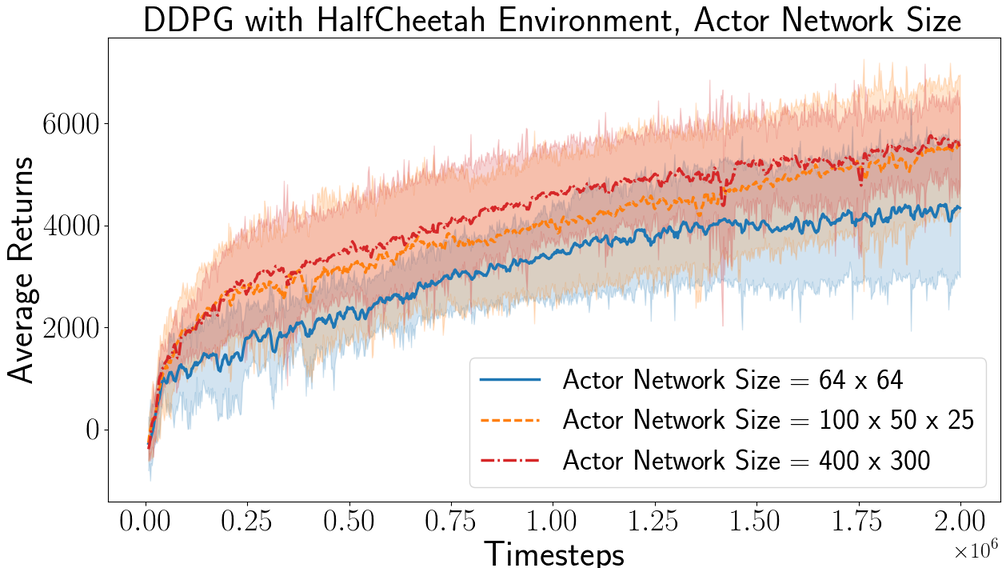
\includegraphics[width=.49\textwidth]{images/ddpg_halfcheetah_policy_size.png}
        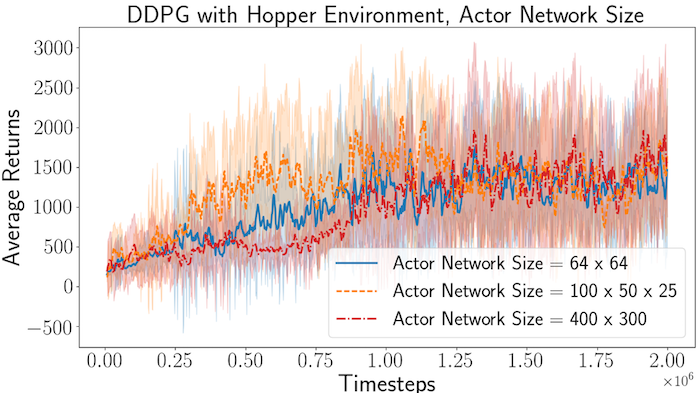
\includegraphics[width=.49\textwidth]{images/ddpg_hopper_policy_size.png}
    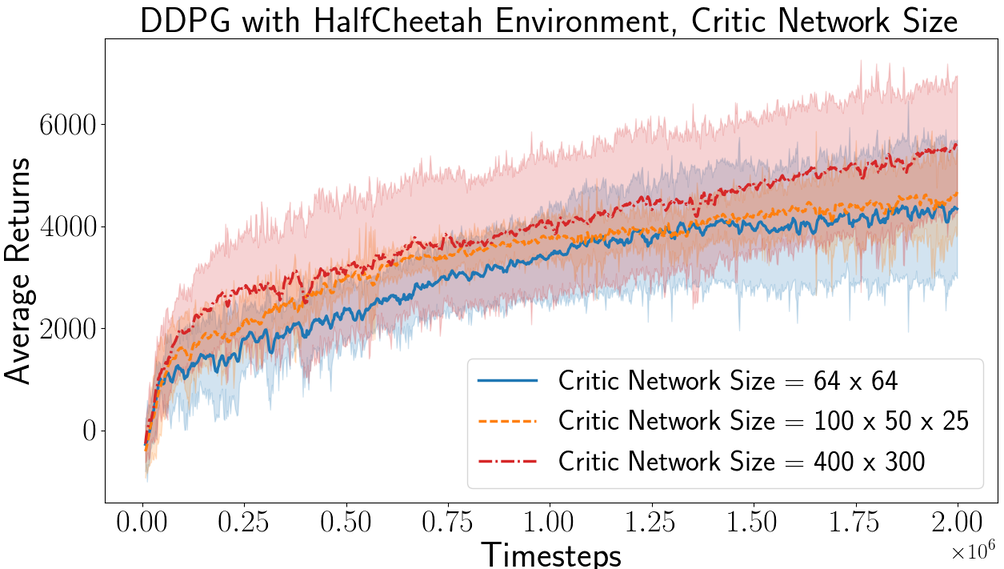
\includegraphics[width=.49\textwidth]{images/ddpg_halfcheetah_value_function_size.png}
        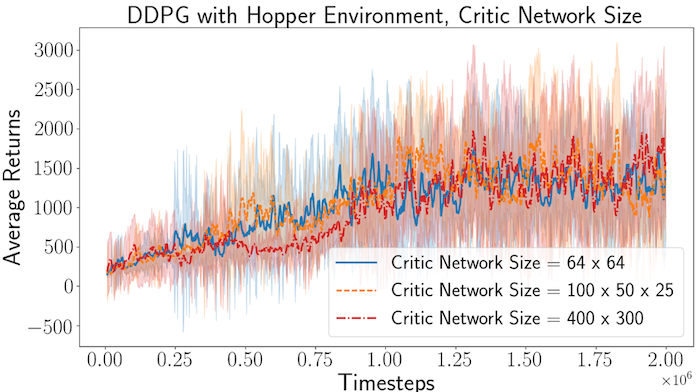
\includegraphics[width=.49\textwidth]{images/ddpg_hopper_value_function_size.png}

    \caption{Policy or Actor Network Architecture experiments for DDPG on HalfCheetah and Hopper Environment}
    \label{fig:ddpgnetwork}
\end{figure}

We further analyze the actor and critic network configurations for use in DDPG. As in default configurations, we first use the ReLU activation function for policy networks, and examine the effect of different activations and network sizes for the critic networks. Similarly, keeping critic network configurations under default setting, we also examine the effect of actor network activation functions and network sizes.


\begin{figure}[H]
    \centering
    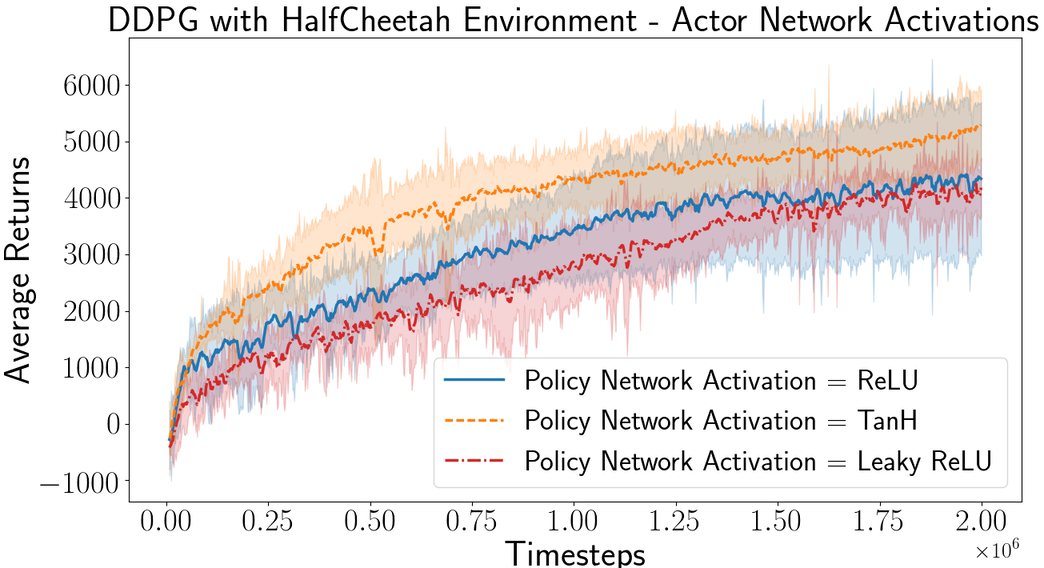
\includegraphics[width=.49\textwidth]{images/ddpg_halfcheetah_policy_activations.png}
    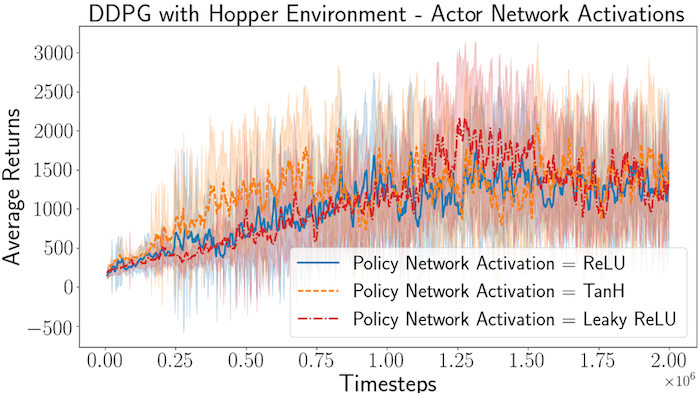
\includegraphics[width=.49\textwidth]{images/ddpg_hopper_policy_activations.png}
        \label{fig:ddpgnetworkact}
\end{figure}

\begin{figure}[H]
    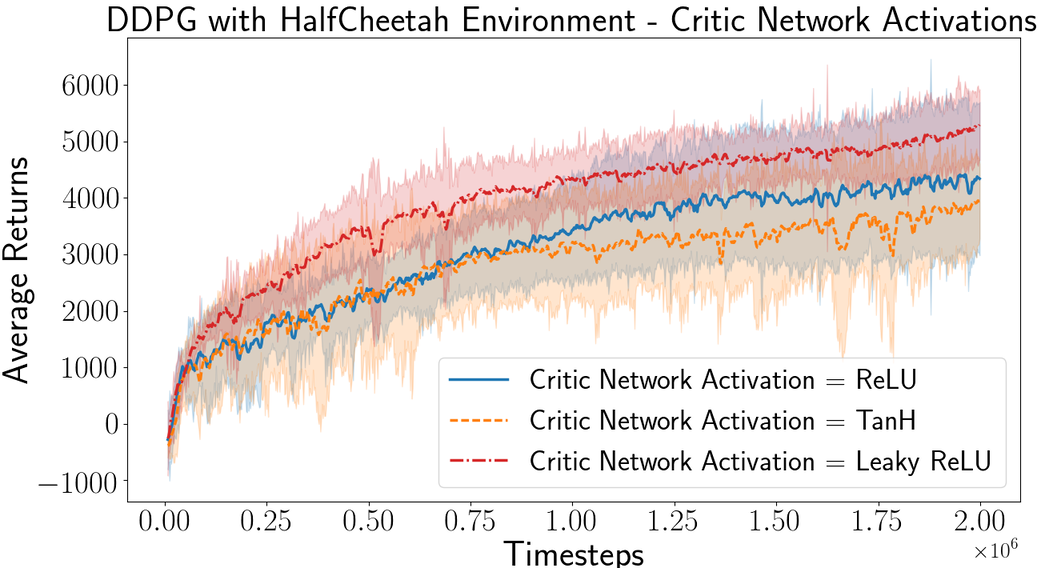
\includegraphics[width=.49\textwidth]{images/ddpg_halfcheetah_value_activations.png}
    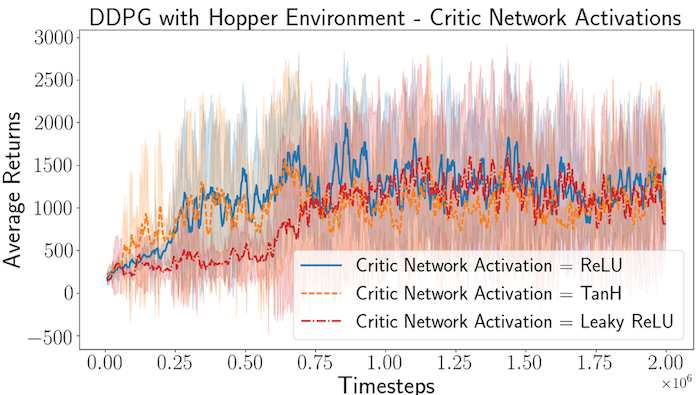
\includegraphics[width=.49\textwidth]{images/ddpg_hopper_value_activations.png}
    \caption{Significance of Value Function or Critic Network Activations for DDPG on HalfCheetah and Hopper Environment}
    \label{fig:ddpgnetworkact2}
\end{figure}


\section{Reward Scaling Parameter in DDPG}

\begin{figure}[H]
    \centering
    \includegraphics[width=.49\textwidth]{"images/Hopper-v1__DDPG,_Reward_Scale,_No_Layer_Norm_"}
    \includegraphics[width=.49\textwidth]{"images/Hopper-v1__DDPG,_Reward_Scale,_Layer_Norm_"}
    \caption{DDPG reward rescaling on Hopper-v1, with and without layer norm.}
    \label{fig:reward_scaling_ddpg2}
\end{figure}

\begin{figure}[H]
    \includegraphics[width=.49\textwidth]{"images/HalfCheetah-v1__DDPG,_Reward_Scale,_Layer_Norm_"}
    \includegraphics[width=.49\textwidth]{"images/HalfCheetah-v1__DDPG,_Reward_Scale,_No_Layer_Norm_"}
    \caption{DDPG reward rescaling on HalfCheetah-v1, with and without layer norm.}
    \label{fig:reward_scaling_ddpg}
\end{figure}

Several related work ~\cite{QPROP,IPG,rllab} have often reported  that for DDPG the reward scaling parameter often needs to be fine-tuned for stabilizing the performance of DDPG. It can make a significant impact in performance of DDPG based on the choice of environment. We examine several reward scaling parameters and demonstrate the effect this parameter can have on the stability and performance of DDPG, based on the HalfCheetah and Hopper environments. Our experiment results, as demonstrated in Figure~\ref{fig:reward_scaling_ddpg} and~\ref{fig:reward_scaling_ddpg2}, show that the reward scaling parameter indeed can have a significant impact on performance. Our results show that, very small or negligible reward scaling parameter can significantly detriment the performance of DDPG across all environments. Furthermore, a scaling parameter of $10$ or $1$ often performs good. Based on our analysis, we suggest that every time DDPG is reported as a baseline algorithm for comparison, the reward scaling parameter should be fine-tuned, specific to the algorithm.


\section{Batch Size in TRPO}

\begin{figure}[H]
    \centering
    \includegraphics[width=.49\textwidth]{"images/Hopper-v1__TRPO,_original,_Batch_Size_"}
    \includegraphics[width=.49\textwidth]{"images/HalfCheetah-v1__TRPO,_original,_Batch_Size_"}
    \caption{TRPO~\cite{TRPO} original code batch size experiments.}
    \label{fig:batch_size_original}
\end{figure}

\begin{figure}[H]
    \centering
    \includegraphics[width=.49\textwidth]{"images/Hopper-v1__TRPO,_baselines,_Batch_Size_"}
    \includegraphics[width=.49\textwidth]{"images/HalfCheetah-v1__TRPO,_baselines,_Batch_Size_"}
    \includegraphics[width=.49\textwidth]{"images/Walker2d-v1__TRPO,_baselines,_Batch_Size_"}
    \includegraphics[width=.49\textwidth]{"images/Reacher-v1__TRPO,_baselines,_Batch_Size_"}
    \caption{TRPO~\cite{PPO} baselines code batch size experiments.}
    \label{fig:batch_size_baselines}
\end{figure}


We run batch size experiments using the original TRPO code~\cite{TRPO} and the OpenAI baselines code~\cite{PPO}. These results can be found in Experiment results in Figure~\ref{fig:batch_size_original} and Figure~\ref{fig:batch_size_baselines}, show that for both HalfCheetah-v1 and Hopper-v1 environments, a batch size of $1024$ for TRPO performs best, while perform degrades consecutively as the batch size is increased.



\section{Random Seeds}

To determine much random seeds can affect results, we run 10 trials total on two environments using the default previously described settings usign the~\cite{QPROP} implementation of DDPG and the~\cite{rllab} version of TRPO. We divide our trials random into 2 partitions and plot them in Figures~\ref{fig:randomseeds_trposup} and Fig~\ref{fig:randomseeds_ddpg_sup}. As can be seen, statistically different distributions can be attained just from the random seeds with the same exact hyperparameters. As we will discuss later, bootstrapping off of the sample can give an idea for how drastic this effect will be, though too small a bootstrap will still not give concrete enough results.

\begin{figure}[H]
    \centering
    \includegraphics[width=0.45\textwidth]{"images/HalfCheetah-v1__TRPO,_Different_Random_Seeds_"}
    \includegraphics[width=0.45\textwidth]{"images/Hopper-v1__TRPO,_Different_Random_Seeds_"}
    \caption{Two different TRPO experiment runs, with same hyperparameter configurations, averaged over two splits of 5 different random seeds. }
    \label{fig:randomseeds_trposup}
\end{figure}


\begin{figure}[H]
    \centering
    \includegraphics[width=0.45\textwidth]{"images/HalfCheetah-v1__DDPG,_Different_Random_Seeds_"}
    \includegraphics[width=0.45\textwidth]{"images/Hopper-v1__DDPG,_Different_Random_Seeds_"}
    \caption{Two different DDPG experiment runs, with same hyperparameter configurations, averaged over two splits of 5 different random seeds. }
    \label{fig:randomseeds_ddpg_sup}
\end{figure}


\section{Choice of Benchmark Continuous Control Environment}


We previously demonstrated that the performance of policy gradient algorithms can be highly biased based on the choice of the environment. In this section, we include further results examining the impact the choice of environment can have. We show that no single algorithm can perform consistenly better in all environments. This is often unlike the results we see with DQN networks in Atari domains, where results can often be demonstrated across a wide range of Atari games. Our results, for example, shows that while TRPO can perform significantly better than other algorithms on the Swimmer environment, it may perform quite poorly n the HalfCheetah environment, and marginally better on the Hopper environment compared to PPO. We demonstrate our results using the OpenAI MuJoCo Gym environments including Hopper, HalfCheetah, Swimmer and Walker environments. It is notable to see the varying performance these algorithms can have even in this small set of environment domains. The choice of reporting algorithm performance results can therefore often be biased based on the algorithm designer's experience with these environments.

\begin{figure}[H]
    \centering
    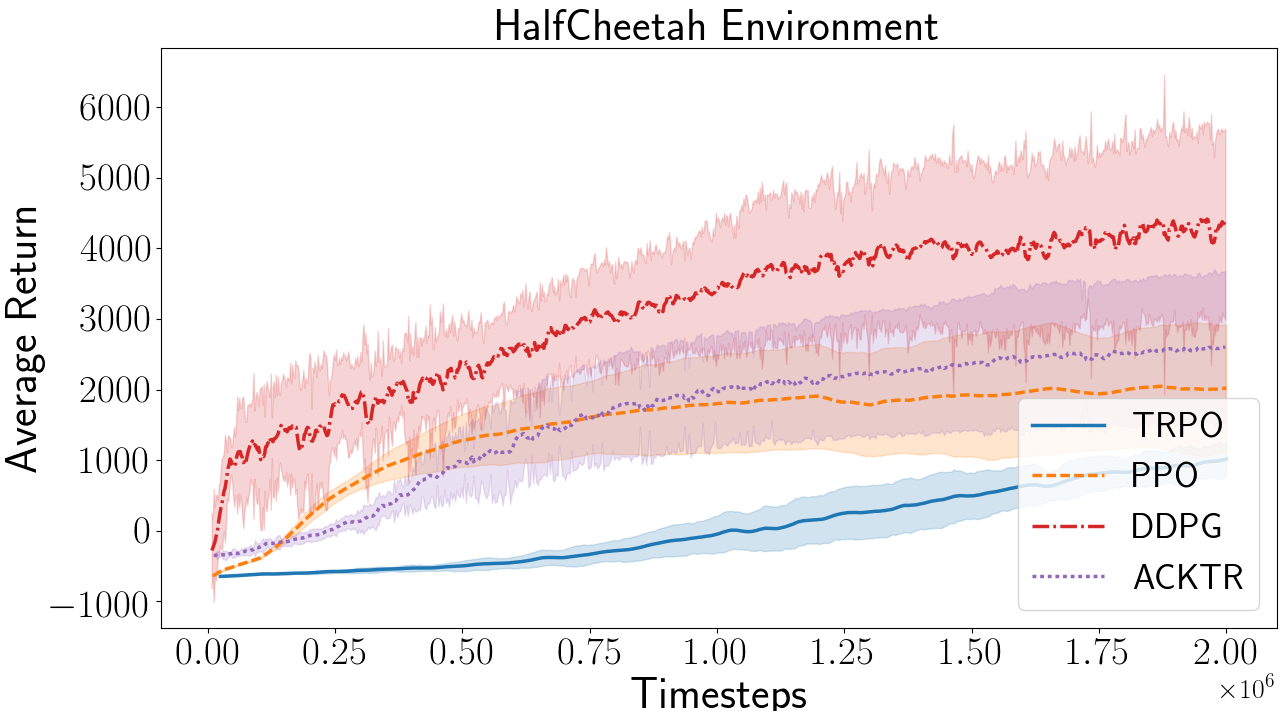
\includegraphics[width=.49\textwidth]{images/HalfCheetah_Env_Algos.png}
    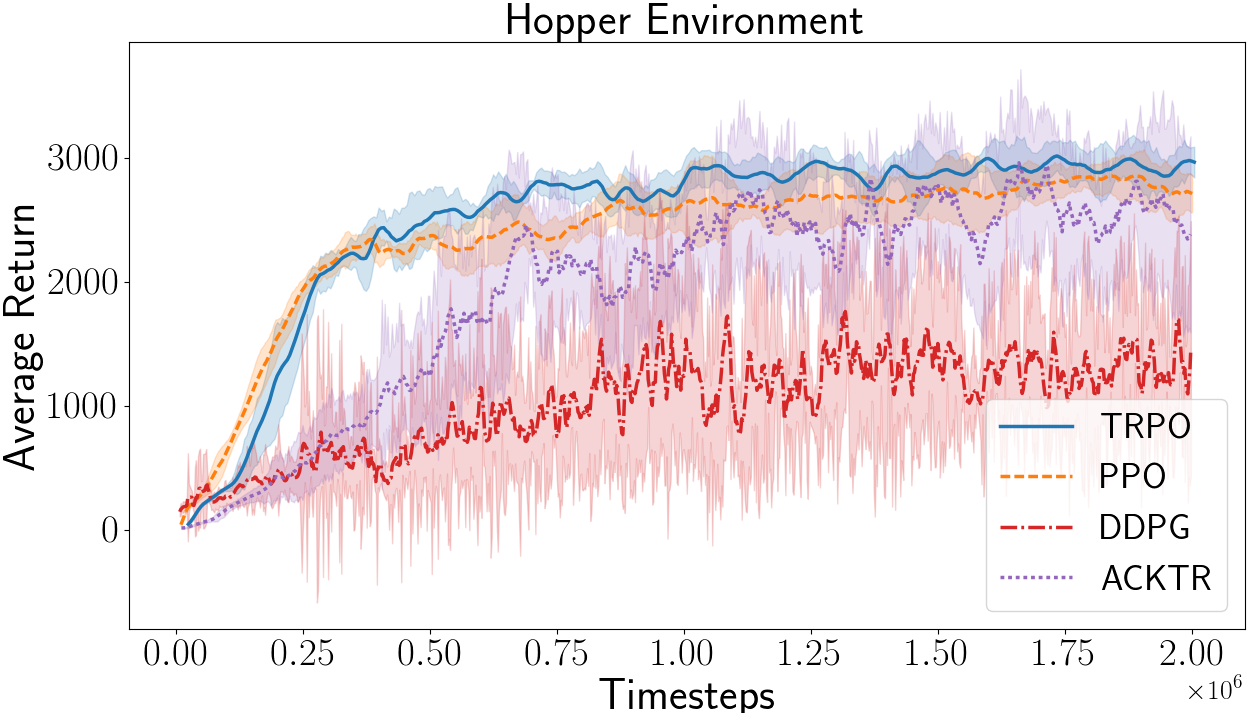
\includegraphics[width=.49\textwidth]{images/Hopper_Env_Algos.png}
\end{figure}

\begin{figure}[H]
    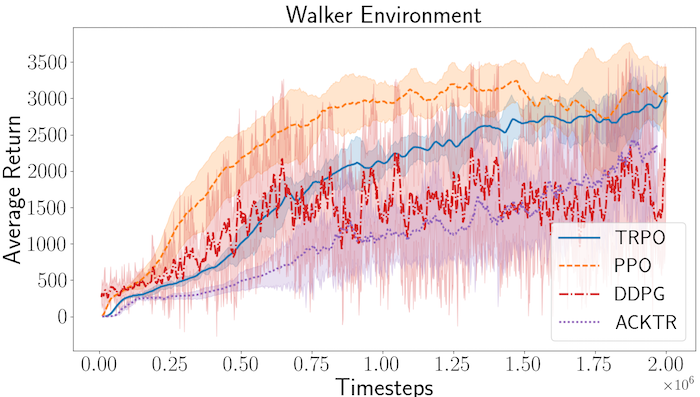
\includegraphics[width=.49\textwidth]{images/Walker_Env_Algos.png}
    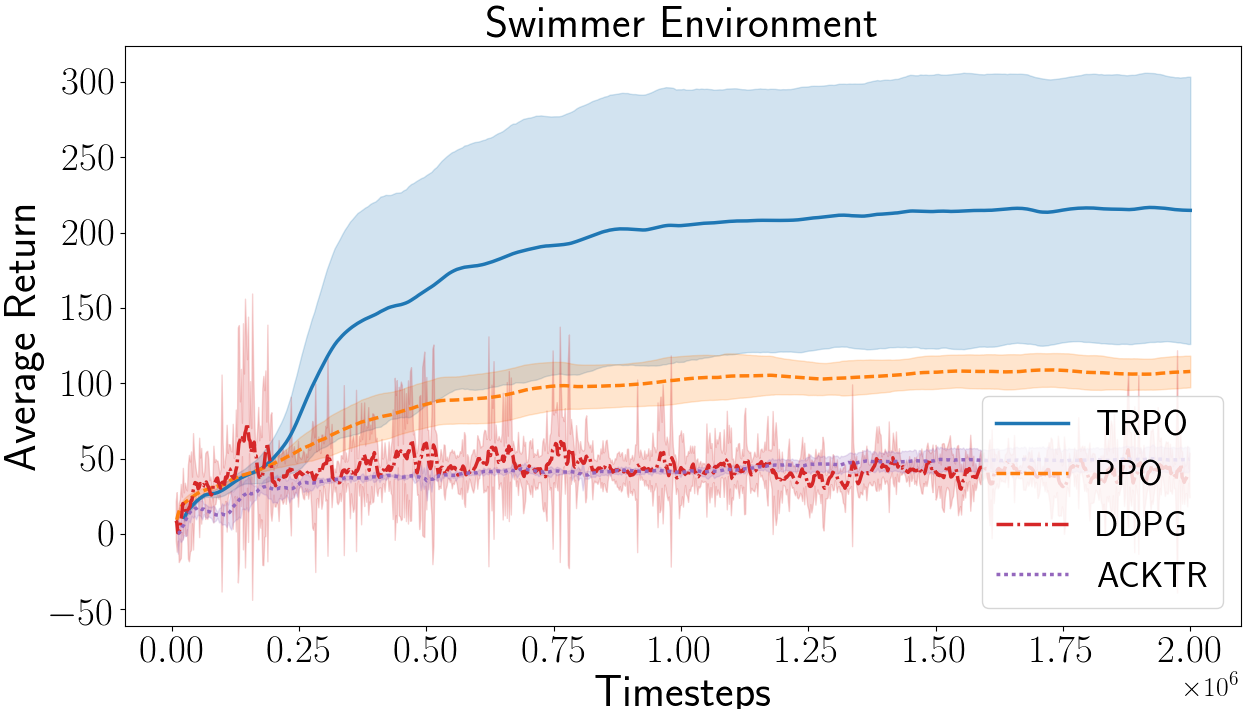
\includegraphics[width=.49\textwidth]{images/Swimmer_Env_Algos.png}
    \caption{Comparing Policy Gradients across various environments}
    \label{fig:halfcheetahenv}
\end{figure}





\section{Codebases}

We include a detailed analysis of performance comparison, with different network structures and activations, based on the choice of the algorithm implementation codebase.

\begin{figure}[H]
    \centering
    \includegraphics[width=.49\textwidth]{"images/HalfCheetah-v1__TRPO,_Original_Code,_Policy_Network_Structure_"}
    \includegraphics[width=.49\textwidth]{"images/Hopper-v1__TRPO,_Original_Code,_Policy_Network_Structure_"}
    \includegraphics[width=.49\textwidth]{"images/HalfCheetah-v1__TRPO,_Original_Code,_Value_Network_Structure_"}
    \includegraphics[width=.49\textwidth]{"images/Hopper-v1__TRPO,_Original_Code,_Value_Network_Structure_"}
    \caption{TRPO Policy and Value Network structure}
    \label{trpo_original}
\end{figure}

\begin{figure}[H]
    \centering
    \includegraphics[width=.49\textwidth]{"images/HalfCheetah-v1__TRPO,_Original_Code,_Policy_Network_Activation_"}
    \includegraphics[width=.49\textwidth]{"images/Hopper-v1__TRPO,_Original_Code,_Policy_Network_Activation_"}
    \includegraphics[width=.49\textwidth]{"images/HalfCheetah-v1__TRPO,_Original_Code,_Value_Network_Activation_"}
    \includegraphics[width=.49\textwidth]{"images/Hopper-v1__TRPO,_Original_Code,_Value_Network_Activation_"}
    \caption{TRPO Policy and Value Network activations.}
    \label{trpo_original_2}
\end{figure}



\begin{figure}[H]
    \centering
    \includegraphics[width=.49\textwidth]{"images/HalfCheetah-v1__TRPO,_rllab,_Policy_Network_Structure_"}
    \includegraphics[width=.49\textwidth]{"images/Hopper-v1__TRPO,_rllab,_Policy_Network_Structure_"}
    \includegraphics[width=.49\textwidth]{"images/HalfCheetah-v1__TRPO,_rllab,_Policy_Network_Activation_"}
    \includegraphics[width=.49\textwidth]{"images/Hopper-v1__TRPO,_rllab,_Policy_Network_Activation_"}
    \caption{TRPO rllab Policy Structure and Activation}
    \label{fig:trpo_rllab}
\end{figure}


\begin{figure}[H]
    \centering
    \includegraphics[width=.49\textwidth]{"images/HalfCheetah-v1__DDPG,_rllab++,_Policy_Network_Structure_"}
    \includegraphics[width=.49\textwidth]{"images/Hopper-v1__DDPG,_rllab++,_Policy_Network_Structure_"}
    \includegraphics[width=.49\textwidth]{"images/Hopper-v1__DDPG,_rllab++,_Value_Network_Structure_"}
    \includegraphics[width=.49\textwidth]{"images/HalfCheetah-v1__DDPG,_rllab++,_Value_Network_Structure_"}

    \caption{DDPG rllab++ Policy and Value Network structure}
    \label{ddpg_rllab_pp}
\end{figure}



\begin{figure}[H]
    \centering
    \includegraphics[width=.49\textwidth]{"images/HalfCheetah-v1__DDPG,_rllab++,_Policy_Network_Activation_"}
    \includegraphics[width=.49\textwidth]{"images/Hopper-v1__DDPG,_rllab++,_Policy_Network_Activation_"}
    \includegraphics[width=.49\textwidth]{"images/HalfCheetah-v1__DDPG,_rllab++,_Value_Network_Activation_"}
    \includegraphics[width=.49\textwidth]{"images/Hopper-v1__DDPG,_rllab++,_Value_Network_Activation_"}
    \caption{DDPG rllab++ Policy and Value Network activations.}
    \label{ddpg_rllab_pp_2}
\end{figure}

Similarly, Figures~\ref{ddpg_rllab} and~\ref{ddpg_rllab_2} show the same network experiments for DDPG with the Theano implementation of rllab code~\cite{rllab}.

\begin{figure}[H]
    \centering
    \includegraphics[width=.49\textwidth]{"images/HalfCheetah-v1__DDPG,_rllab,_Policy_Network_Structure_"}
    \includegraphics[width=.49\textwidth]{"images/Hopper-v1__DDPG,_rllab,_Policy_Network_Structure_"}
    \includegraphics[width=.49\textwidth]{"images/Hopper-v1__DDPG,_rllab,_Value_Network_Structure_"}
    \includegraphics[width=.49\textwidth]{"images/HalfCheetah-v1__DDPG,_rllab,_Value_Network_Structure_"}
    \caption{DDPG rllab Policy and Value Network structure}
    \label{ddpg_rllab}
\end{figure}


\begin{figure}[H]
    \centering
    \includegraphics[width=.49\textwidth]{"images/HalfCheetah-v1__DDPG,_rllab,_Policy_Network_Activation_"}
    \includegraphics[width=.49\textwidth]{"images/Hopper-v1__DDPG,_rllab,_Policy_Network_Activation_"}
    \includegraphics[width=.49\textwidth]{"images/HalfCheetah-v1__DDPG,_rllab,_Value_Network_Activation_"}
    \includegraphics[width=.49\textwidth]{"images/Hopper-v1__DDPG,_rllab,_Value_Network_Activation_"}
    \caption{DDPG rllab Policy and Value Network activations.}
    \label{ddpg_rllab_2}
\end{figure}


Often in related literature, there is different baseline codebase people use for implementation of algorithms. One such example is for the TRPO algorithm. It is a commonly used policy gradient method for continuous control tasks, and there exists several implementations from OpenAI Baselines \cite{plappert2017parameter}, OpenAI rllab \cite{rllab} and the original TRPO codebase \cite{TRPO}. In this section, we perform an analysis of the impact the choice of algorithm codebase can have on the performance. Figures \ref{trpo_original} and \ref{trpo_original_2} summarizes our results with TRPO policy network and value networks, using the original TRPO codebase from \cite{TRPO}. Figure~\ref{fig:trpo_rllab} shows the results using the rllab implementation of TRPO using the same hyperparameters as our default experiments aforementioned. Note, we use a linear function approximator rather than a neural network due to the fact that the Tensorflow implementation of OpenAI rllab doesn't provide anything else. We note that this is commonly used in other works~\cite{rllab,thirdperson}, but may cause differences in performance. Furthermore, we leave out our value function network experiments due to this.

\begin{figure}[H]
    \centering
    \includegraphics[width=.49\textwidth]{"images/HalfCheetah-v1__DDPG,_Codebase_Comparison_"}
    \includegraphics[width=.49\textwidth]{"images/Hopper-v1__DDPG,_Codebase_Comparison_"}
    \caption{DDPG codebase comparison using our default set of hyperparameters (as used in other experiments).}
    \label{fig:ddpg_codebase}
\end{figure}

\begin{figure}[H]
    \centering
    \includegraphics[width=.49\textwidth]{"images/HalfCheetah-v1__TRPO,_Codebase_Comparison_"}
    \includegraphics[width=.49\textwidth]{"images/Hopper-v1__TRPO,_Codebase_Comparison_"}
    \caption{TRPO codebase comparison using our default set of hyperparameters (as used in other experiments).}
    \label{fig:trpo_codebase}
\end{figure}


Figure~\ref{fig:trpo_codebase} shows a comparison of the TRPO implementations using the default hyperparamters as specified earlier in the supplemental. Note, the exception is that we use a larger batch size for rllab and original TRPO code of 20k samples per batch, as optimized in a second set of experiments. Figure~\ref{ddpg_rllab_pp} and~\ref{ddpg_rllab_pp_2} show the same network experiments for DDPG with the rllab++ code~\cite{QPROP}. We can then compare the performance of the algorithm across 3 codebases (keeping all hyperparameters constant at the defaults), this can be seen in Figure~\ref{fig:ddpg_codebase}.









\section{Significance}

Our full results from significance testing with difference metrics can be found in Table~\ref{tab:significance_cheetah} and Table~\ref{tab:singificance_hopper}. Our bootstrap mean and confidence intervals can be found in Table~\ref{tab:bootstrap}. Bootstrap power analysis can be found in Table~\ref{tab:power}. To performance significance testing, we use our 5 sample trials to generate a bootstrap with 10k bootstraps. From this confidence intervals can be obtained. For the $t$-test and KS-test, the average returns from the 5 trials are sorted and compared using the normal 2-sample versions of these tests. Scipy ( \url{https://docs.scipy.org/doc/scipy-0.14.0/reference/generated/scipy.stats.ks_2samp.html}, \url{https://docs.scipy.org/doc/scipy/reference/generated/scipy.stats.ttest_ind.html}) and Facebook Boostrapped (\url{https://github.com/facebookincubator/bootstrapped}) are used for the KS test, $t$-test, and bootstrap analysis. For power analysis, we attempt to determine if a sample is enough to game the significance of a 25\% lift. This is commonly used in A/B testing~\cite{tuffery2011data}.

\begin{table}[H]
    \centering
    \scriptsize{\begin{tabular}{|c|c|c|c|c|}
    \hline
         - &DDPG&ACKTR&TRPO&PPO  \\
         \hline
         DDPG& - &\shortstack{$t=1.85,p=0.102$\\$KS=0.60,p=0.209$\\61.91 \% (-32.27 \%, 122.99 \%)}&\shortstack{$t=4.59,p=0.002$\\$KS=1.00,p=0.004$\\301.48 \% (150.50 \%, 431.67 \%)}&\shortstack{$t=2.67,p=0.029$\\$KS=0.80,p=0.036$\\106.91 \% (-37.62 \%, 185.26 \%)} \\
         \hline
         ACKTR&\shortstack{$t=-1.85,p=0.102$\\$KS=0.60,p=0.209$\\-38.24 \% (-75.42 \%, -15.19 \%)}&-&\shortstack{$t=2.78,p=0.024$\\$KS=0.80,p=0.036$\\147.96 \% (30.84 \%, 234.60 \%)}&\shortstack{$t=0.80,p=0.448$\\$KS=0.60,p=0.209$\\27.79 \% (-67.77 \%, 79.56 \%)}\\
         \hline
         TRPO&\shortstack{$t=-4.59,p=0.002$\\$KS=1.00,p=0.004$\\-75.09 \% (-86.44 \%, -68.36 \%)}&\shortstack{$t=-2.78,p=0.024$\\$KS=0.80,p=0.036$\\-59.67 \% (-81.70 \%, -46.84 \%) }&-&\shortstack{$t=-2.12,p=0.067$\\$KS=0.80,p=0.036$\\-48.46 \% (-81.23 \%, -32.05 \%) }\\
         \hline
         PPO&\shortstack{$t=-2.67,p=0.029$\\$KS=0.80,p=0.036$\\-51.67 \% (-80.69 \%, -31.94 \%) }&\shortstack{$t=-0.80,p=0.448$\\$KS=0.60,p=0.209$\\-21.75 \% (-75.99 \%, 11.68 \%) }&\shortstack{$t=2.12,p=0.067$\\$KS=0.80,p=0.036$\\94.04 \% (2.73 \%, 169.06 \%) }&-\\
         \hline
    \end{tabular}}
    \caption{HalfCheetah Significance values and metrics for different algorithms. Rows in cells are: sorted 2-sample $t$-test, Kolmogorov-Smirnov test, bootstrap A/B comparison \% difference with 95\% confidence bounds.}
    \label{tab:significance_cheetah}
\end{table}


\begin{table}[H]
    \centering
    \scriptsize{\begin{tabular}{|c|c|c|c|c|}
    \hline
         - &DDPG&ACKTR&TRPO&PPO  \\
         \hline
         DDPG&-&\shortstack{$t=-1.41,p=0.196$\\$KS=0.60,p=0.209$\\-35.92 \% (-85.62 \%, -5.38 \%) }&\shortstack{$t=-2.58,p=0.033$\\$KS=0.80,p=0.036$\\-44.96 \% (-78.82 \%, -20.29 \%) }&\shortstack{$t=-2.09,p=0.070$\\$KS=0.80,p=0.036$\\-39.90 \% (-77.12 \%, -12.95 \%) }\\
         \hline
         ACKTR&\shortstack{$t=1.41,p=0.196$\\$KS=0.60,p=0.209$\\56.05 \% (-87.98 \%, 123.15 \%) }&-&\shortstack{$t=-1.05,p=0.326$\\$KS=0.60,p=0.209$\\-14.11 \% (-37.17 \%, 9.11 \%) }&\shortstack{$t=-0.42,p=0.686$\\$KS=0.40,p=0.697$\\-6.22 \% (-31.58 \%, 18.98 \%) }\\
         \hline
         TRPO&\shortstack{$t=2.58,p=0.033$\\$KS=0.80,p=0.036$\\81.68 \% (-67.76 \%, 151.64 \%) }&\shortstack{$t=1.05,p=0.326$\\$KS=0.60,p=0.209$\\16.43 \% (-27.92 \%, 41.17 \%) }&-&\shortstack{$t=2.57,p=0.033$\\$KS=0.60,p=0.209$\\9.19 \% (2.37 \%, 15.58 \%) }\\
         \hline
         PPO&\shortstack{$t=2.09,p=0.070$\\$KS=0.80,p=0.036$\\66.39 \% (-67.80 \%, 130.16 \%) }&\shortstack{$t=0.42,p=0.686$\\$KS=0.40,p=0.697$\\6.63 \% (-33.54 \%, 29.59 \%) }&\shortstack{$t=-2.57,p=0.033$\\$KS=0.60,p=0.209$\\-8.42 \% (-14.08 \%, -2.97 \%) }&-\\
         \hline
    \end{tabular}}
    \caption{Hopper Significance values and metrics for different algorithms. Rows in cells are: sorted 2-sample $t$-test, Kolmogorov-Smirnov test, bootstrap A/B comparison \% difference with 95\% confidence bounds.}
    \label{tab:singificance_hopper}
\end{table}


\begin{table}[H]
    \centering
    \scriptsize{\begin{tabular}{|c|c|c|c|c|}
    \hline
         - &DDPG&ACKTR&TRPO&PPO  \\
         \hline
         DDPG&-&\shortstack{$t=-1.03,p=0.334$\\$KS=0.40,p=0.697$\\-30.78 \% (-91.35 \%, 1.06 \%) }&\shortstack{$t=-4.04,p=0.004$\\$KS=1.00,p=0.004$\\-48.52 \% (-70.33 \%, -28.62 \%) }&\shortstack{$t=-3.07,p=0.015$\\$KS=0.80,p=0.036$\\-45.95 \% (-70.85 \%, -24.65 \%) }\\
         \hline
         ACKTR&\shortstack{$t=1.03,p=0.334$\\$KS=0.40,p=0.697$\\44.47 \% (-80.62 \%, 111.72 \%) }&-&\shortstack{$t=-1.35,p=0.214$\\$KS=0.60,p=0.209$\\-25.63 \% (-61.28 \%, 5.54 \%) }&\shortstack{$t=-1.02,p=0.338$\\$KS=0.60,p=0.209$\\-21.91 \% (-61.53 \%, 11.02 \%) }\\
         \hline
         TRPO&\shortstack{$t=4.04,p=0.004$\\$KS=1.00,p=0.004$\\94.24 \% (-22.59 \%, 152.61 \%) }&\shortstack{$t=1.35,p=0.214$\\$KS=0.60,p=0.209$\\34.46 \% (-60.47 \%, 77.32 \%) }&-&\\
         \hline
         PPO&\shortstack{$t=3.07,p=0.015$\\$KS=0.80,p=0.036$\\85.01 \% (-31.02 \%, 144.35 \%) }&\shortstack{$t=1.02,p=0.338$\\$KS=0.60,p=0.209$\\28.07 \% (-65.67 \%, 71.71 \%) }&\shortstack{$t=-0.57,p=0.582$\\$KS=0.40,p=0.697$\\-4.75 \% (-19.06 \%, 10.02 \%) }&-\\
         \hline
    \end{tabular}}
    \caption{Walker2d Significance values and metrics for different algorithms. Rows in cells are: sorted 2-sample $t$-test, Kolmogorov-Smirnov test, bootstrap A/B comparison \% difference with 95\% confidence bounds.}
    \label{tab:singificance_walker}
\end{table}


\begin{table}[H]
    \centering
    \scriptsize{\begin{tabular}{|c|c|c|c|c|}
    \hline
         - &DDPG&ACKTR&TRPO&PPO  \\
         \hline
         DDPG&-&\shortstack{$t=-2.18,p=0.061$\\$KS=0.80,p=0.036$\\-36.44 \% (-61.04 \%, -6.94 \%) }&\shortstack{$t=-4.06,p=0.004$\\$KS=1.00,p=0.004$\\-85.13 \% (-97.17 \%, -77.95 \%) }&\shortstack{$t=-8.33,p=0.000$\\$KS=1.00,p=0.004$\\-70.41 \% (-80.86 \%, -56.52 \%) }\\
         \hline
         ACKTR&\shortstack{$t=2.18,p=0.061$\\$KS=0.80,p=0.036$\\57.34 \% (-80.96 \%, 101.11 \%) }&-&\shortstack{$t=-3.69,p=0.006$\\$KS=1.00,p=0.004$\\-76.61 \% (-90.68 \%, -70.06 \%) }&\shortstack{$t=-8.85,p=0.000$\\$KS=1.00,p=0.004$\\-53.45 \% (-62.22 \%, -47.30 \%) }\\
         \hline
         TRPO&\shortstack{$t=4.06,p=0.004$\\$KS=1.00,p=0.004$\\572.61 \% (-73.29 \%, 869.24 \%) }&\shortstack{$t=3.69,p=0.006$\\$KS=1.00,p=0.004$\\327.48 \% (165.47 \%, 488.66 \%) }&-&\shortstack{$t=2.39,p=0.044$\\$KS=0.60,p=0.209$\\99.01 \% (28.44 \%, 171.85 \%) }\\
         \hline
         PPO&\shortstack{$t=8.33,p=0.000$\\$KS=1.00,p=0.004$\\237.97 \% (-59.74 \%, 326.85 \%) }&\shortstack{$t=8.85,p=0.000$\\$KS=1.00,p=0.004$\\114.80 \% (81.85 \%, 147.33 \%) }&\shortstack{$t=-2.39,p=0.044$\\$KS=0.60,p=0.209$\\-49.75 \% (-78.58 \%, -36.43 \%) }&-\\
         \hline
    \end{tabular}}
    \caption{Swimmer Significance values and metrics for different algorithms. Rows in cells are: sorted 2-sample $t$-test, Kolmogorov-Smirnov test, bootstrap A/B comparison \% difference with 95\% confidence bounds.}
    \label{tab:singificance_swimmer}
\end{table}


\begin{table}[H]
    \centering
    \scriptsize{\begin{tabular}{|c|c|c|c|c|}
    \hline
         Environment&DDPG&ACKTR&TRPO&PPO  \\
         \hline
         HalfCheetah-v1&5037.26 (3664.11, 6574.01)&3888.85 (2288.13, 5131.96)&1254.55 (999.52, 1464.86)& 3043.1 (1920.4, 4165.86)\\
         \hline
         Hopper-v1&1632.13 (607.98, 2370.21)&2546.89 (1875.79, 3217.98)&2965.33 (2854.66, 3076.00)&2715.72 (2589.06, 2847.93)\\
         Walker2d-v1&1582.04 (901.66, 2174.66)&2285.49 (1246.00, 3235.96)&3072.97 (2957.94, 3183.10)&2926.92 (2514.83, 3361.43)\\
         \hline
         Swimmer-v1&31.92 (21.68, 46.23)&50.22 (42.47, 55.37)&214.69 (141.52, 287.92)&107.88 (101.13, 118.56)\\
         \hline
    \end{tabular}}
    \caption{Envs bootstrap mean and 95\% confidence bounds}
    \label{tab:bootstrap}
\end{table}


\begin{table}[H]
    \centering
    \begin{tabular}{|c|c|c|c|c|}
    \hline
         Environment&DDPG&ACKTR&TRPO&PPO  \\
         \hline
         HalfCheetah-v1&\shortstack{100.00 \% \\ 0.00 \% \\ 0.00 \%}&\shortstack{79.03 \%\\11.53 \% \\ 9.43 \%}&\shortstack{79.47 \% \\ 20.53 \% \\ 0.00 \%}&\shortstack{61.07 \% \\ 10.50 \% \\ 28.43 \%}\\
         \hline
         Hopper-v1&\shortstack{60.90 \%\\10.00 \% \\ 29.10 \%}&\shortstack{79.60 \% \\ 11.00 \% \\ 9.40 \%}&\shortstack{0.00 \% \\ 100.00 \% \\ 0.00 \%}&\shortstack{0.00 \% \\ 100.00 \% \\ 0.00 \%}\\
         \hline
         Walker2d-v1&\shortstack{89.50 \%\\0.00 \% \\ 10.50 \%}&\shortstack{60.33 \% \\ 9.73 \% \\ 29.93 \%}&\shortstack{0.00 \% \\ 100.00 \% \\ 0.00 \%}&\shortstack{59.80 \% \\ 31.27 \% \\ 8.93 \%}\\
         \hline
         Swimmer-v1&\shortstack{89.97 \%\\0.00 \% \\ 10.03 \%}&\shortstack{59.90 \% \\ 40.10 \% \\ 0.00 \%}&\shortstack{89.47 \% \\ 0.00 \% \\ 10.53 \%}&\shortstack{40.27 \% \\ 59.73 \% \\ 0.00 \%}\\
         \hline
    \end{tabular}
    \caption{Power Analysis for predicted significance of 25\% lift. Rows in cells are: \% insignificant simulations,\% positive significant, \% negative significant.}
    \label{tab:power}
\end{table}





% % REFERENCES
% % \section{References}
% \bibliographystyle{aaai}
% \bibliography{bibliography}
